
\chapter{Spatial and temporal relationships between GTHA data sources} \label{ch:spatial_and_temporal_relationships_between_urban_data}

\section{Introduction: data sources used in the GTHA housing market database} \label{sec:intro_data_sources}

%TODO add chapter introduction
List data sources used in Teranet database.

\section{Description of data sources} \label{sec:description_of_data_sources}

This section describes different data sources combined into the GTHA housing market database.

\subsection{Teranet's dataset of land registration records} \label{subsec:teranet_description}

%TODO rewrite description for Teranet dataset
Teranet dataset of real estate transactions recorded in the Province of Ontario holds a wealth of information on the housing market of Ontario, but is very limited in the number of available attributes.
The dataset can be augmented by joining additional attributes from various data sources, such as Census or TTS survey, based on spatial and/or temporal relationships.
These relationships are best organized in the form of a relational database based on a database management system, such as PostgreSQL .
Teranet dataset plays an integral part in the proposed GTHA housing market database, design and implementation of which is the primary focus of this Master Thesis.

\subsection{Census of Canada} \label{subsec:census_description}

%TODO finish description of Census
One of the major sources of demographic and statistical data in Canada are the datasets collected under the national Census program.
Statistics Canada collects every five years the national Census of Canada and disseminates the information by a range of geographic units, also referred to as "Census geography"\cite{MapandDataLibrary2019}.
Census geography follows a certain hierarchy defined by Statistics Canada, with the largest top-level divisions being provinces and territories, lowest-tier divisions to which census data is disseminated are Dissemination Areas (DAs)\cite{StatisticsCanada2018}.
Statistics Canada defines a dissemination area as a small area composed of one or more neighbouring dissemination blocks, roughly uniform in population size targeted from 400 to 700 persons to avoid data suppression\cite{StatisticsCanada2015}.

\subsection{Transportation Tomorrow Survey (TTS)} \label{subsec:tts_description}

%TODO finish description of TTS
Another major source of information for most transportation planning studies concerned with Southern Ontario is the Transportation Tomorrow Survey (TTS)\cite{DataManagementGroup2014}, an origin destination travel survey.
The Transportation Tomorrow Survey (TTS), undertaken every five years since 1986, is a cooperative effort by local and provincial government agencies to collect information about urban travel in southern Ontario.
TTS represents a retrospective survey of travel taken by every member (age 11 or over) of the household during the day previous to the telephone or web contact.
The information collected and the method of collection has remained relatively consistent over the seven surveys and includes characteristics of the household, characteristics of each person in the household, and details of the trips taken by each member of the household, including details on any trips taken by transit\cite{Ashby2018}.

The finest level of spatial aggregation available through iDRS is that of the Traffic Zone also referred to as Traffic Analysis Zone (TAZ).
TTS data has been collected for changing TAZ boundaries or in other words, different zone systems due to growing population and expanding extents of the survey in the GTHA region over the years.
To make the TTS data consistent for comparing over all years from 1986 to 2016, the data management group (DMG), the custodian of the dataset derived from TTS, made all surveys available in the 2001 zone system, for convenience of researchers.
Any zone system could have been chosen for that matter.
Not as a rule, but the TAZs roughly follow census tract boundaries, which are slightly bigger than DA boundaries.
Overview of the traffic zones and their boundaries: http://dmg.utoronto.ca/survey-boundary-files#tts

\subsection{DMTI data} \label{subsec:dmti_data}

%TODO add some description of DMTI datasets (EPOI, land use)

\subsection{Detailed land use information from geography department} \label{subsec:detailed_land_use_from_geogrpahy_department}

%TODO add some description of the detailed land use obtained from the geography department

\section{Spatial relationships between datasets} \label{sec:spatial_relationships}

%TODO finish section
This section introduces the spatial relationships between the datasets used in the GTHA housing market database.

\subsection{Accessibility as a measure of land use-transportation relationship} \label{subsec:accessibility}

While traffic studies have primarily focused on mobility, or the ease of moving,
LUT models operationalize the transportation-land use relationship by incorporating measures of accessibility with the process of locating activities, typically assuming that households wish to locate in areas with higher accessibility to employment, shopping, or entertainment opportunities.
Similarly, firms are assumed to locate in areas with higher accessibility to labour markets.
Accessibility measures the situation of a location relative to other activities or opportunities (work, shopping, etc.) distributed in space and can be an important determinant of price in LUT models where land and floor space markets are considered explicitly\cite{Iacono2008}.
When measuring changes in relative accessibility, it is usually approximated by some measure of access to the transportation network, such as travel time or distance.

Land use component is usually integrated into the accessibility measure through congested network travel times.
However, when studying the relationship between transportation facilities and property values, results may vary based on whether travel time or travel distance is used as a measure of accessibility\cite{Sherry1999}.
To simulate the changes in accessibility, metropolitan regions are usually broken down into a set of small geographic zones, similar (or in many cases identical) to the set of zones used for regional travel forecasting.
Changes to relative accessibility of a location can thus be estimated as changes in zone-to-zone travel times in a travel network\cite{Iacono2008}.

\subsection{Breakdown of an urban region} \label{subsec:breakdown_of_urban_region}

%TODO add maps with DA and TAZ boundaries overlayed
Most urban areas are divided into zones or planning areas on the basis of maintaining similar population sizes and following built or natural boundaries like roads or rivers.
For many research purposes, it would be beneficial to use multiple data sources, such as when characterizing the interaction between transportation and land use.
To reveal heterogeneity of the systems it is necessary to use the highest spatial and temporal resolution possible.
This dictates the need for the smallest spatial scales at which different survey data is available.
For example for census data, a dissemination area is the smallest standard geographic area for which all census data are disseminated.

One of the major sources of demographic and statistical data in Canada are the datasets collected under the national Census program.
Statistics Canada collects every five years the national Census of Canada and disseminates the information by a range of geographic units, also referred to as "Census geography"\cite{MapandDataLibrary2019}.
Census geography follows a certain hierarchy defined by Statistics Canada, with the largest top-level divisions being provinces and territories, lowest-tier divisions to which census data is disseminated are Dissemination Areas (DAs)\cite{StatisticsCanada2018}.
Statistics Canada defines a dissemination area as a small area composed of one or more neighbouring dissemination blocks, roughly uniform in population size targeted from 400 to 700 persons to avoid data suppression\cite{StatisticsCanada2015}.

Another major source of information for most transportation planning studies concerned with Southern Ontario is the Transportation Tomorrow Survey (TTS)\cite{DataManagementGroup2014}, an origin destination travel survey.
The Transportation Tomorrow Survey (TTS), undertaken every five years since 1986, is a cooperative effort by local and provincial government agencies to collect information about urban travel in southern Ontario.
TTS represents a retrospective survey of travel taken by every member (age 11 or over) of the household during the day previous to the telephone or web contact.
The information collected and the method of collection has remained relatively consistent over the seven surveys and includes characteristics of the household, characteristics of each person in the household, and details of the trips taken by each member of the household, including details on any trips taken by transit\cite{Ashby2018}.

The finest level of spatial aggregation available through iDRS is that of the Traffic Zone also referred to as Traffic Analysis Zone (TAZ).
TTS data has been collected for changing TAZ boundaries or in other words, different zone systems due to growing population and expanding extents of the survey in the GTHA region over the years.
To make the TTS data consistent for comparing over all years from 1986 to 2016, the data management group (DMG), the custodian of the dataset derived from TTS, made all surveys available in the 2001 zone system, for convenience of researchers.
Any zone system could have been chosen for that matter.
Not as a rule, but the TAZs roughly follow census tract boundaries, which are slightly bigger than DA boundaries.
Overview of the traffic zones and their boundaries: http://dmg.utoronto.ca/survey-boundary-files#tts

We used the 2001 zone system to model travel times for the GTHA on EMME for all TTS years based on the origin-destination trip data collected in the survey.
The travel time data was used to create further transportation accessibility variables.
%TODO streamline info about breakdown of an urban region, move info about spatial units to the next subsection.

\subsection{Spatial units used by the data sources in the GTHA housing market database} \label{subsec:spatial_units_used_in_database}

%TODO write subsection about the spatial units used

\section{Temporal relationships between datasets} \label{sec:termporal_relationships_between_datasets}

\subsection{Temporal spans at which different urban data sources are available} \label{subsec:temporal_scales}

%TODO write a section about temporal scales
Figure~\ref{fig:temporal_spans} presents temporal spans of the data sources used in the GTHA housing market database.
\begin{figure}[hbt!]
    \centering
    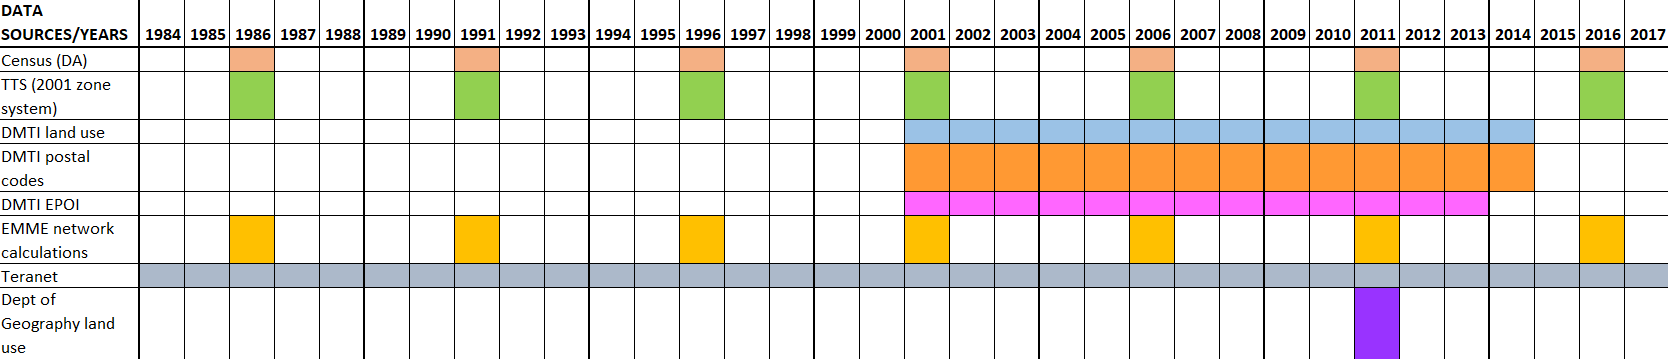
\includegraphics[width=1\linewidth,trim=0 0 0 0,clip]{temporal_spans.png}
    \caption{Temporal spans of the data sources used in the GTHA housing market database.}
    \label{fig:temporal_spans}
\end{figure}

\subsection{Possible approaches to matching temporal spans to relate data sources} \label{subsec:possible_approaches_to_match_temporal_spans}

Teranet and Census / TTS variables can be matched in a number of ways:

\begin{enumerate}
    \item Direct match with appropriate Teranet subsets
    \begin{itemize}
        \item use subsets of Teranet records from the Census / TTS years and match only with data directly recorded for that year
        \item for example, take a subset of Teranet records from 2016 and match it with 2016 Census / TTS variables
        \item technically, any date span can be specified when creating a Teranet subset, but in this case, appropriate Census / TTS variables must be selected manually
        \item benefits:
        \begin{itemize}
            \item precision of match: variables from Census would be composed of the actual values produced by the survey, rather than an interpolation based on assumptions
            \item flexibility of use: a new Census table can be added and its variables can be match with appropriate Teranet records via simple SQL queries
        \end{itemize}
        \item disadvantages:
        \begin{itemize}
            \item limited match: only Teranet data from Census years can be used, records from between Census years cannot be matched with the Census vairables
            \item hard to generalize SQL queries: need custom SQL queries to match data to different tables, several queries to match Teranet data from different Census years
        \end{itemize}
    \end{itemize}
    \item Interpolation of discrete Census / TTS variables
    \begin{itemize}
        \item discrete Census / TTS variables can be turned into continuous via interpolation
        \item Teranet records can be matched to real recorded and interpolated values by year, or finer time scale
        \item benefits:
        \begin{itemize}
            \item most Teranet records used: all Teranet records within the Census / TTS range can be used (within the interpolation region)
            \item closest match: closest temporal match between Teranet records and Census / TTS variables
            \item precise, if correctly assessed: in the case where correct assumptions are made while interpolating values, the most precise match
        \end{itemize}
        \item disadvantages:
        \begin{itemize}
            \item more assumptions: additional assumptions need to be made about the dynamics of each Census / TTS variables between Census years
            \item inaccurate, if incorrectly assessed: in case of incorrect assumptions, there is a risk of lower accuracy compared with other matching methods
            \item interpolated rather then recorded: Teranet values from non-Census years will be matched to variables that are interpolated rather then recorded
            \item more data pre-processing needed: each Census / TTS variable needs to be processed in order to produce interpolated values
        \end{itemize}
    \end{itemize}
    \item Assign temporal spans for each Census / TTS survey as new features to Teranet records
    \begin{itemize}
        \item each Census / TTS survey can be assigned a temporal span of 5 years representing a group of Teranet records to which its variables can be matched
        \item Teranet records are matched by year, each year would yield an appropriate Census or TTS variable from an appropriate temporal span
        \item for example, the Census of 2016 would have a temporal span of 2014--2018, and thus a Teranet record from 2015 would be matched to variables from 2016 Census.
        \item Census of 1991 would have a temporal span of 1989--1993, and thus a Teranet record from 1993 would be matched with variables from 1991 Census.
        \item TTS survey would be matched in a similar manner
        \item benefits:
        \begin{itemize}
            \item most Teranet records used: all Teranet / TTS records that fall within the specified temporal spans range can be matched to appropriate Census / TTS variables
            \item recorded rather than interpolated: Teranet records are matched to actual recorded Census / TTS values
            \item avoid interpolation assumptions: since no interpolation is performed, no additional assumptions are needed
            \item no additional data pre-processing: all matching is done through an "adapter" table, original Census / TTS variables do not need to be changed
        \end{itemize}
        \item disadvantages:
        \begin{itemize}
            \item step-change in Census / TTS variables: when matching Teranet sources from non-Census years, instead of using interpolation, same Census / TTS variables are used for a group of 5 years centered at each Census year
            \item varying accuracy: accuracy of match further away from the Census years (+/- 2 years) probably will be lower.
            In addition, there would be a step change from every +2 to -2 Census year (i.e., 1998 to 1999)
            \item need new foreign keys: additional features specifying the temporal spans of Census / TTS variables to years for each Teranet record needs to be added to the Teranet table to facilitate temporal integrity of the joining operations
            \item Census and TTS tables need to be in a "tidy" data format, with each variable being a column, and each observation being a row.
            Year of Census and TTS needs to be encoded as a separate variable `year`, `year` and `dauid` or `taz_o` becoming the primary keys of TTS and Census tables.
            In a case of a large number of variables such transformation makes Census table "long" instead of "wide".
        \end{itemize}
    \end{itemize}
\end{enumerate}


\subsection{Matching temporal scales to facilitate linking datasets} \label{subsec:matching_temporal_scales}
%TODO write a subsection about matching temporal scales

\section{Chapter summary} \label{sec:data_sources_summary}
Different data sources use different spatial and temporal scales, and that's what we are going to address with data prep and the database.
%TODO write chapter summary
